\documentclass{article}
\usepackage[letterpaper, margin=0.95in]{geometry}
\usepackage[T1]{fontenc}
\usepackage{titleps}
\usepackage{parskip}
\usepackage{booktabs}
\usepackage{graphicx}
\usepackage{xcolor}
\usepackage{microtype}
\usepackage[hidelinks]{hyperref}

\newpagestyle{ruled}
{\sethead{CMU 16-831}{Intro to Robot Learning}{Fall 2026}\headrule
  \setfoot{}{}{}}
\pagestyle{ruled}
\renewcommand\makeheadrule{\color{black}\rule[-.75\baselineskip]{\linewidth}{0.4pt}}

\begin{document}

\begin{center}
    {\Large Assignment 1: Imitation Learning} \\
    \vspace{.25cm}
    \textbf{Andrew ID:} \texttt{shritas} \\
    \textbf{Collaborators:} \texttt{Claude code for running scripts and formatting}
\end{center}

% \textit{Generative AI tools such as ChatGPT are viewed as collaborators in this course, acknowledge accordingly.}

\section{Behavioral Cloning (10 pt)}

\subsection{Part 2 (1.5 pt)}
\begin{table}[!h]
  \centering
  \caption{Mean and standard deviation of expert return over two trajectories, for each environment.}
  \begin{tabular}{cccccc}
    \toprule
    Metric/Env & Ant-v2 & Humanoid-v2 & Walker2d-v2 & Hopper-v2 & HalfCheetah-v2 \\
    \midrule
    Mean  & 4713.65 & 10344.52 & 5566.85 & 3772.67 & 4205.78 \\
    Std.  & 12.20 & 20.98 & 9.24 & 1.95 & 83.04 \\
    \bottomrule
  \end{tabular}
  \label{tab:p2}
\end{table}

\subsection{Part 3 (5 pt)}

Hyperparameters: default network size (2 layers, 64 units), default learning rate (5e-3), 
  \texttt{eval\_batch\_size}=5000 (collecting 5 trajectories), 
  \texttt{num\_agent\_train\_steps\_per\_iter}=2000 (randomly sampled from the full dataset). \\
I set evaluation batch size to calculate mean and variance of return over 5 trajectories. 
I also increased the number of training steps to get a better fit over expert data performance. 
I did not need to change the train batch size to achieve close to expert performance for the ant task, 
but the humanoid task performance did not improve significantly with more training steps.
\begin{table}[htbp]
  \centering
  \caption{BC vs.\ expert return on Ant-v2 and Humanoid-v2. }
  \begin{tabular}{ccccc}
    \toprule
    Env   & \multicolumn{2}{c}{Ant-v2} & \multicolumn{2}{c}{Humanoid-v2} \\
    \midrule
    Metric & Mean  & Std.  & Mean  & Std. \\
    Expert & 4713.65 & 12.20 & 10344.52 & 20.98 \\
    BC    & 4540.18 & 117.38 & 277.59 & 55.74 \\
    \bottomrule
  \end{tabular}
  \label{tab:p3}
\end{table}

\subsection{Part 4 (3 pt)}
Hypothesis: Fewer, longer rollouts should outperform more, shorter rollouts with the same total transitions. \\
I generated a fixed 2000-transition dataset considering two types of episode length and rollout combos: (2$\times$1000 vs.\ 10$\times$200) to test this hypothesis. \\
The result did not support this hypothesis -- more, shorter rollouts gave a higher mean return (498.03 vs.\ 277.59) but far higher variance (std 202.91 vs.\ 55.74). 
This could be due to longer rollouts encountering similar set of states while using expert policy, while shorter rollouts are 
initialized randomly and explore more of the state space, leading to a better fit and higher reward.
\begin{figure}[!h]
  \centering
  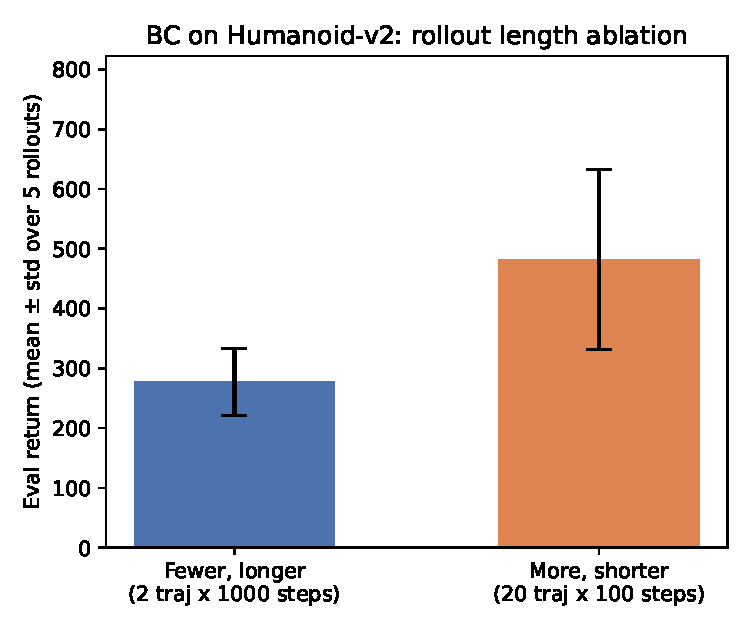
\includegraphics[width=0.4\columnwidth]{figure_placeholder.pdf}
  \caption{Hypothesis: on the higher-dimensional Humanoid-v2 task, fewer, longer expert rollouts would train a better BC policy than more, shorter ones with the same total transitions}
  \label{fig:p4}
\end{figure}

\subsection{Part 5 (0.5 pt)}
Fu et al., ``Mobile ALOHA'' (CoRL 2024), clones mobile bimanual tasks like cooking and cabinet manipulation from whole-body human teleoperation demos. 
A main IL risk from this homework is encountering covariate shift, where the learned policy visits states it has not seen in expert data set and performs poorly. 
This risk still applies to the paper's methodology, as the learned policy may encounter states not seen in the human teleoperation demos.

\newpage
\section{DAgger (5 pt)}

\subsection{Part 2 (5 pt)}
Hyperparameters: all defaults (2-layer/64-unit MLP, learning rate 5e-3, \texttt{num\_agent\_\allowbreak train\_steps\_\allowbreak per\_iter}=1000, \texttt{train\_\allowbreak batch\_size}=100, \texttt{batch\_\allowbreak size}=1000 expert-relabeled data aggregated per iteration), except \texttt{eval\_\allowbreak batch\_size}=5000 (5 eval trajectories) and \texttt{n\_iter}=10 DAgger iterations. \\
On Ant-v2, DAgger outperforms behavior cloning and approaches expert performance. On iteration 5, the mean reward jumps down and the std deviation jumps up, which may be due to a bad episode while iterating. 
On Humanoid-v2, DAgger improves the mean return from 289 to 491 but is still much lower than expert performance (10344). This could be due to the high-dimensional state space of Humanoid-v2, which may need a deeper MLP policy to learn the expert policy.
\begin{figure}[!h]
  \centering
  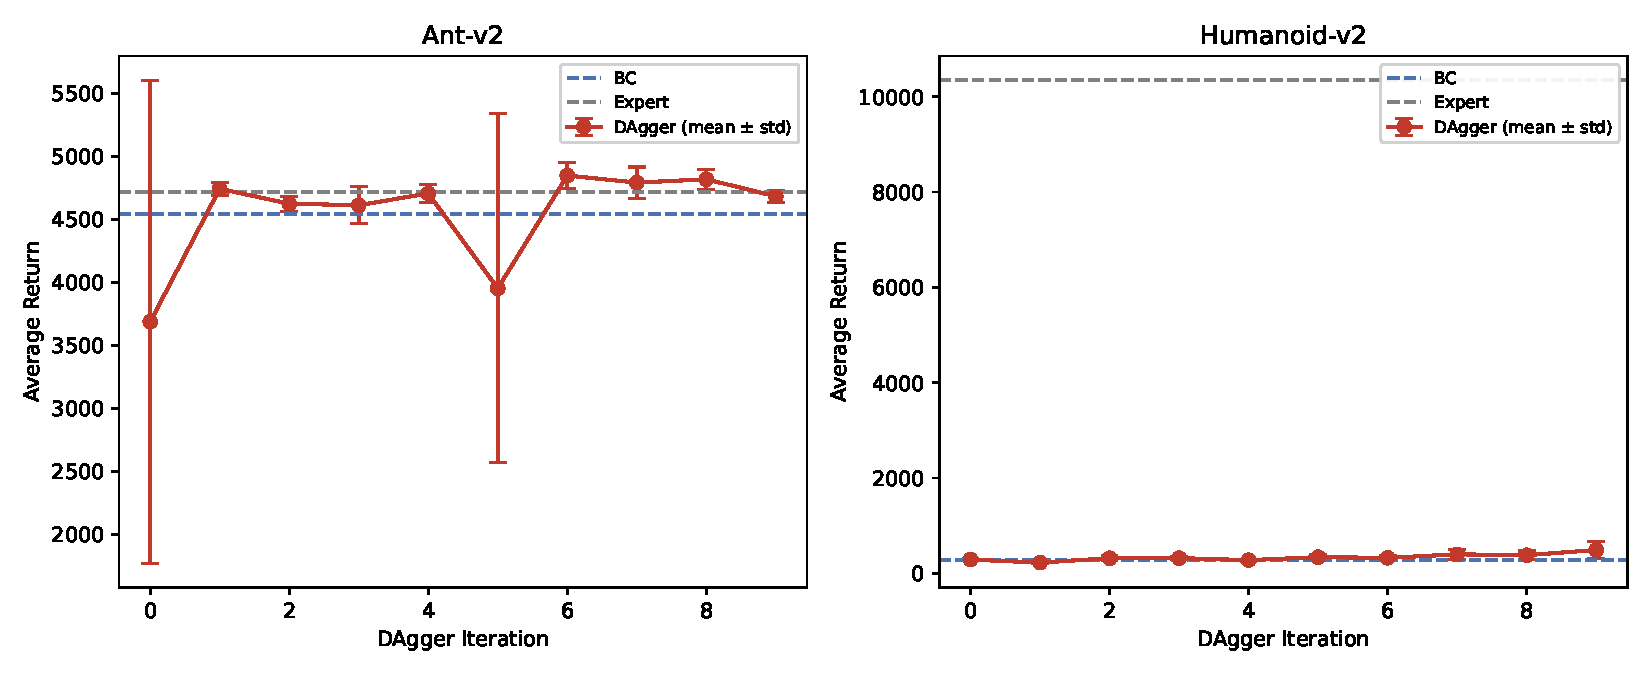
\includegraphics[width=\columnwidth]{figure2_dagger.pdf}
  \caption{DAgger learning curves (mean return vs.\ iteration, with error bars for std deviation) on Ant-v2 (left) and Humanoid-v2 (right), 
  BC and Expert performance are blue-grey and grey lines.}
  \label{fig:p5}
\end{figure}


\end{document}
